\chapter{Attention in Transformers}
The core mechanism that differentiates the Transformer from all previous architectures is \textbf{self-attention}. This component, first introduced in the paper "Attention is All You Need", is what allows the model to dynamically weigh the importance of different parts of the input sequence. Understanding this mechanism is the key to understanding both the ViT's $O(N^2)$ computational problem \cite{ref2} and its elegant, "built-in" solution: attention-based token pruning.

\section{What is Attention? The QKV Analogy}

At its heart, the attention mechanism is a function that calculates a weighted average. For every token in the input sequence (e.g., every image patch), it asks a question: "Given my own identity, how much 'attention' should I pay to every *other* token in this sequence?" \cite{ref2}

To answer this, the model uses an analogy from information retrieval, creating three distinct vectors from each token's embedding \cite{ref20}:
\begin{itemize}
    \item \textbf{Query (Q):} A vector representing the token's "question" or "search request." It asks, "What kind of information am I looking for?"
    \item \textbf{Key (K):} A vector representing the token's "label" or "identity." It responds to queries, saying, "This is the information I have."
    \item \textbf{Value (V):} A vector representing the token's *actual content* or "meaning." This is the information that is retrieved once a match is made.
\end{itemize}

The entire operation is captured in a single, elegant formula known as \textbf{Scaled Dot-Product Attention} \cite{ref2}:
$$\text{Attention}(Q, K, V) = \text{softmax} \left( \frac{Q K^T}{\sqrt{d_k}} \right) V$$
This formula is executed in a few key steps, as illustrated in Figure \ref{fig:scaled_dot_product}:

\begin{enumerate}
    \item \textbf{Score:} The model calculates a "similarity score" by taking the dot product of one token's \textbf{Query} vector with every other token's \textbf{Key} vector. This is the $Q K^T$ (Query-Key Transpose) matrix multiplication.
    
    \item \textbf{Scale and Normalize:} The raw scores are passed through a $\text{softmax}$ function, which converts them into a set of positive weights that sum to 1.0. These are the "attention probabilities."
    
    Crucially, before the softmax, the scores are divided by $\sqrt{d_k}$, the square root of the key/query dimension. This \textbf{"scaling" factor} is vital for stable training. Why? As the dimension $d_k$ grows, the dot product values $Q K^T$ also grow larger in magnitude. These large values push the $\text{softmax}$ function into its "saturated" regions (where the input is a large positive or negative number). In these regions, the gradient becomes almost zero, making it impossible for the model to learn. This is the "vanishing gradient" problem. Dividing by $\sqrt{d_k}$ scales the dot products back, keeping their variance stable and ensuring the $\text{softmax}$ operates in its active, high-gradient region.
    
    \item \textbf{Weighted Sum:} The model multiplies these normalized attention weights (the output of the softmax) by the corresponding \textbf{Value} vectors. The result is a new, context-rich embedding for that token, which is a weighted blend of all other tokens in the sequence.
\end{enumerate}

When this operation is performed where Q, K, and V are all derived from the *same* input sequence (i.e., the sequence attends to itself), it is called \textbf{self-attention}. When multiple such "attention heads" are run in parallel, it becomes the \textbf{Multi-Head Self-Attention (MHSA)} block found in the ViT encoder \cite{ref2, ref18}.

\begin{figure}[h!]
    \centering
    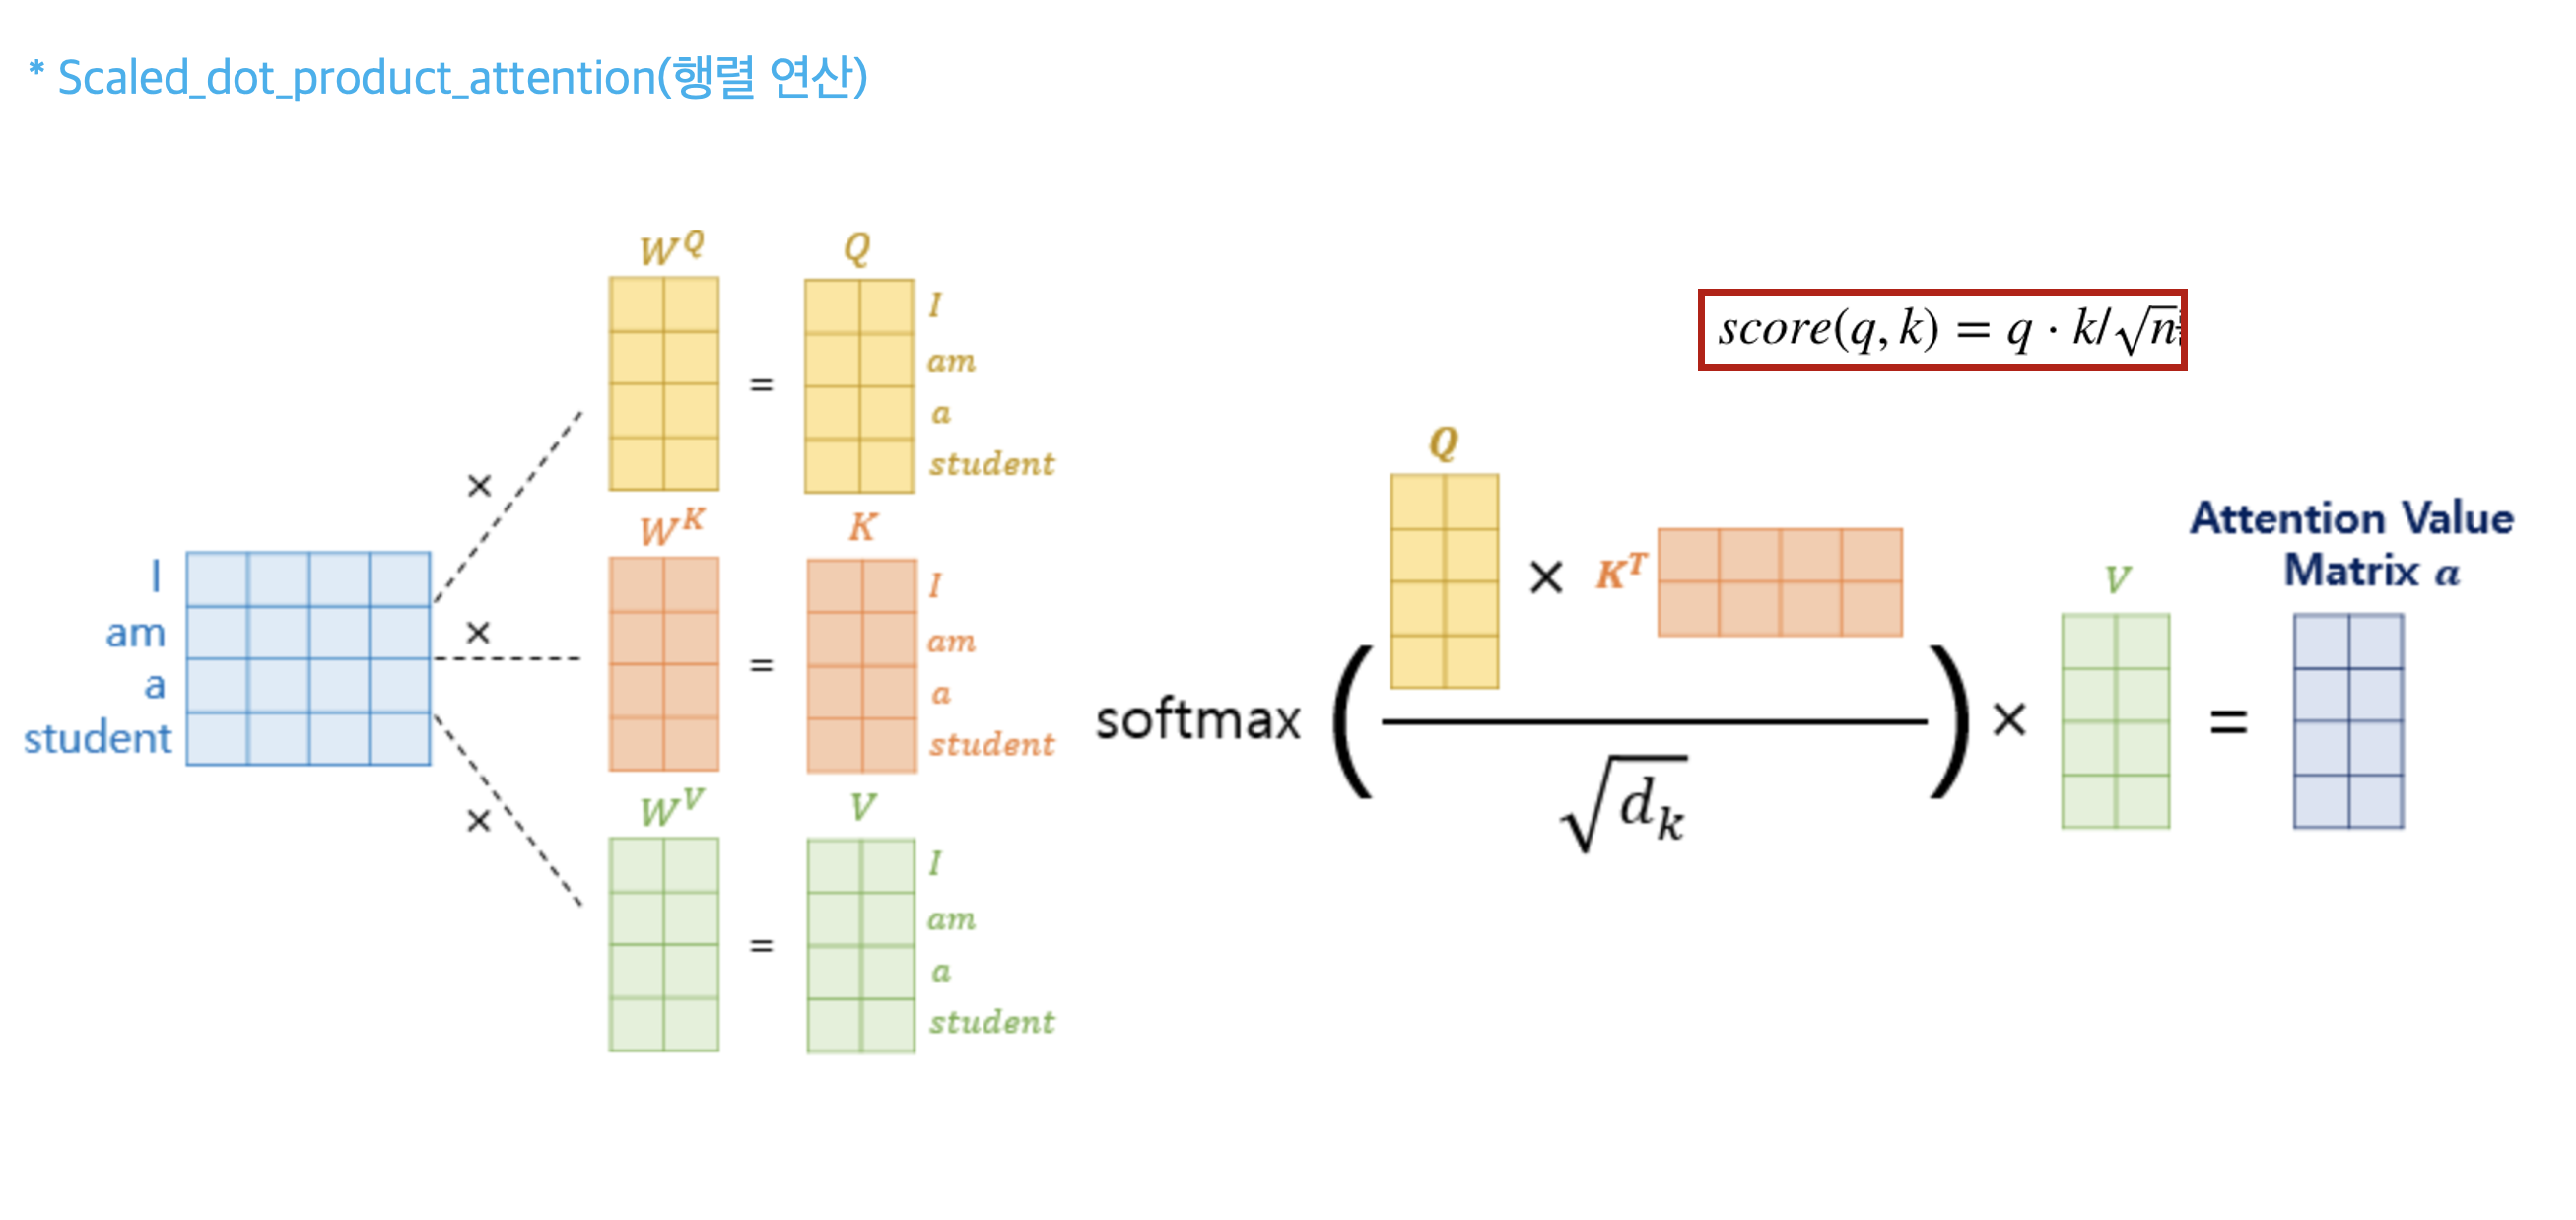
\includegraphics[width=\textwidth]{images/scaled_dot_product.png}
    \caption{Scaled Dot-Product Attention }
    \label{fig:scaled_dot_product}
\end{figure}

\section{Why Attention-Based Token Selection is Relevant}

The $O(N^2)$ complexity of self-attention comes from the very first step: calculating the $N \times N$ matrix of attention scores. The central insight for ViT acceleration is that this $N \times N$ matrix, while computationally expensive, is also an incredibly rich source of information.

The final classification in a ViT is often based on only a small subset of the most informative tokens \cite{ref3, ref6}. Many tokens, such as those representing a uniform background, contribute very little to the final decision \cite{ref13}. The model, in effect, "learns" to ignore them.

This "importance" is not a mystery—it is explicitly encoded in the attention weights. If a token consistently receives low attention scores from other tokens (especially from the important \texttt{CLS} token), it is, by the model's own definition, "uninformative."

Therefore, the attention matrix itself is the most natural and efficient metric for pruning. Instead of training a separate, complex "prediction module" to guess which tokens are important \cite{ref3}, we can simply use the attention scores that the model *already computes* as a direct, non-parametric importance score \cite{ref4}. This makes attention-based pruning highly relevant for hardware acceleration, as it adds almost zero algorithmic overhead while directly attacking the $O(N^2)$ computational problem.

\begin{table}[h!]
    \centering
    \begin{tabular}{|l|l|l|}
        \hline
        \textbf{Pruning Metric} & \textbf{How it Works} & \textbf{Hardware/Compute Cost} \\
        \hline
        \textbf{Attention-Based} & Aggregates attention scores & \textbf{Very Low} \\
        (This Project) & from the existing MHSA block \cite{ref4}. & (Reuses existing calculation). \\
        \hline
        \textbf{Predictor-Based} & Trains a separate, lightweight & \textbf{Medium} \\
        (e.g., DynamicViT) & neural network to predict & (Adds new layers and FLOPs \\
        & token importance \cite{ref3}. & for the predictor module). \\
        \hline
    \end{tabular}
    \caption{Comparison of different token importance metrics.}
    \label{table:pruning_metrics}
\end{table}

\section{Implementation in the HLS C++ Code}

The provided HLS code implements a highly effective and hardware-friendly version of this attention-based pruning. The entire process is contained within the \texttt{transformer\_block} function and its sub-routines.

\subsection{Step 1: Calculating Importance}
After the \texttt{mha\_block} computes the full $HEADS \times SEQ\_LEN \times SEQ\_LEN$ attention matrix (\texttt{attn\_probs}), the \texttt{transformer\_block} immediately calls:
\begin{verbatim}
compute_attention_importance(attn_probs, importance);
\end{verbatim}
Looking at the \texttt{compute\_attention\_importance} function, we can see exactly how the importance score is derived:
\begin{verbatim}
for (int j = 0; j < SEQ_LEN; ++j) {
    float sum = 0.0f;
    for (int h = 0; h < HEADS; ++h) {
        sum += attn_probs[h][j];  // attention from CLS to token j
    }
    importance[j] = sum / HEADS;
}
\end{verbatim}
This is a non-parametric approach that uses the \textbf{CLS token's attention} as the metric \cite{ref4}. It calculates an "importance score" for each token \texttt{j} by averaging, across all heads, the attention it received from the CLS token (\texttt{token 0}). This is a standard and effective method, as the CLS token's job is to aggregate all information necessary for classification.

\subsection{Step 2: Creating the Pruning Mask}
Next, the \texttt{transformer\_block} calls:
\begin{verbatim}
make_prune_mask(importance, new_mask, 0.80f);
\end{verbatim}
The \texttt{make\_prune\_mask} function takes the \texttt{importance} scores and the hard-coded \texttt{keep\_ratio} of 0.80 (meaning 20\% of tokens will be pruned, though this is set to ~15\% in our abstract's final configuration). It then finds the score of the $k$-th most important token (where $k = 0.80 \times SEQ\_LEN$) and uses this score as a threshold. The code performs this "Top-K" search using a \textbf{Partial Selection Sort}.

This choice of algorithm is a deliberate hardware-design decision. In a pure software context, one might use a faster algorithm like \texttt{std::nth\_element} (which often uses an Introselect, a hybrid of Quickselect and Heapselect). However, such algorithms are poorly suited for HLS for several reasons:
\begin{itemize}
    \item \textbf{Recursive algorithms} (like QuickSort/Quickselect) are not synthesizable by HLS.
    \item \textbf{Data-dependent latency} (as seen in Quickselect) is highly undesirable in a pipelined hardware accelerator, which relies on deterministic, fixed-cycle operations.
    \item \textbf{Hardware overkill:} Full sorting networks (like Bitonic or Merge Sort) are HLS-synthesizable but would consume a massive amount of hardware resources (comparators and registers) and are unnecessary, as we only need the $k$-th element, not the entire sorted list.
\end{itemize}

The \textbf{Partial Selection Sort} used in the code is the preferred HLS approach because it is:
\begin{enumerate}
    \item \textbf{Simple:} The logic is just a nested loop with a comparison, which maps easily to simple HLS control logic.
    \item \textbf{Deterministic:} Its latency is fixed and predictable ($O(N \cdot K)$), which allows the HLS scheduler to integrate it perfectly into a larger pipeline.
    \item \textbf{Resource-Efficient:} It requires minimal hardware (a simple loop and swap logic) and reuses the same logic for each iteration, making it very "cheap" in terms of FPGA resources.
\end{enumerate}

\subsection{Step 3: Skipping Computation}
This mask is the key to the hardware acceleration. In the second half of the \texttt{transformer\_block}, all computation is guarded by this mask:
\begin{verbatim}
LN2_T:
    for (int t = 0; t < SEQ_LEN; ++t)
        if (active_mask[t])
            layer_norm(seq_out[t], ln2_out[t],...);

MLP_T:
    for (int t = 0; t < SEQ_LEN; ++t)
        if (active_mask[t])
            mlp_block_token(ln2_out[t], mlp_out[t], blk);
\end{verbatim}
This \texttt{if (active\_mask[t])} check is the entire hardware pruning mechanism. It instructs the HLS compiler to synthesize logic that \textbf{dynamically skips} all LayerNorm and MLP computations for tokens that were marked as "pruned." This "token skipping" \cite{ref10} directly reduces the computational load (FLOPs) of the second half of the Transformer block.

\section{Architectural Choice: Skipping vs. Reordering}

The "skip" strategy implemented in this code is a critical and deliberate hardware-design choice. When implementing dynamic pruning, there are two main architectural strategies, which present a trade-off between hardware complexity and computational efficiency.

\begin{table}[h!]
    \centering
    \begin{tabular}{|l|l|l|}
        \hline
        \textbf{Strategy} & \textbf{Description} & \textbf{Hardware Implication} \\
        \hline
        \textbf{Skipping (Masking)} & Keeps the $N \times D$ matrix structure. & \textbf{Simple}. Requires only an \texttt{if} \\
        (Our HLS Code) & Uses a boolean mask to "skip" & check. Avoids all data reordering. \\
        & computation on pruned tokens \cite{ref10}. & \\
        \hline
        \textbf{Reordering (Compaction)} & Physically shuffles the data, & \textbf{Complex}. Requires a "Token \\
        (e.g., \cite{ref6, ref13}) & creating a new, smaller $N' \times D$ & Dropping Module" (TDM) \cite{ref5} to \\
        & dense matrix. & manage irregular memory access \cite{ref4}. \\
        \hline
    \end{tabular}
    \caption{Comparison of hardware-level pruning strategies.}
    \label{table:pruning_strategies}
\end{table}

The "Reordering" strategy is, in theory, more computationally efficient, as the subsequent processing loops only need to iterate to $N'$, not $N$. However, this comes at a massive cost in hardware complexity. It requires an "on-the-fly" data shuffling and reordering module \cite{ref5, ref6}, which is very difficult to implement efficiently in HLS and can cause its own latency bottlenecks \cite{ref12}.

The HLS code provided wisely chooses the \textbf{Skipping} strategy. By simply using an \texttt{if} statement, it avoids all the complex hardware logic for data reordering. This is an excellent example of algorithm-hardware codesign: the "skip" algorithm is chosen specifically because it maps perfectly to a simple, efficient, and high-performance HLS implementation.